\documentclass[10pt,a4paper]{ctexart}

\usepackage[a4paper,margin=1.35cm,headheight=14pt,footskip=18pt]{geometry}
\usepackage{fontspec}
\usepackage{xeCJK}
\usepackage{graphicx}
\usepackage{xcolor}
\usepackage{booktabs}
\usepackage{tabularx}
\usepackage{array}
\usepackage{enumitem}
\usepackage{hyperref}
\usepackage{fancyhdr}
\usepackage[most]{tcolorbox}
\usepackage{amsmath}
\usepackage{pifont}
\usepackage{microtype}

\setCJKmainfont{Noto Sans CJK SC}
\setCJKsansfont{Noto Sans CJK SC}
\setmainfont{Noto Sans CJK SC}
\setsansfont{Noto Sans CJK SC}
\setmonofont{DejaVu Sans Mono}

\definecolor{navy}{HTML}{102A43}
\definecolor{blue}{HTML}{2563EB}
\definecolor{bluebg}{HTML}{EFF6FF}
\definecolor{green}{HTML}{0F766E}
\definecolor{greenbg}{HTML}{ECFDF5}
\definecolor{amber}{HTML}{B45309}
\definecolor{amberbg}{HTML}{FFFBEB}
\definecolor{red}{HTML}{B91C1C}
\definecolor{redbg}{HTML}{FEF2F2}
\definecolor{slate}{HTML}{486581}
\definecolor{line}{HTML}{CBD5E1}
\definecolor{light}{HTML}{F8FAFC}

\hypersetup{
  colorlinks=true,
  linkcolor=navy,
  urlcolor=blue,
  pdftitle={近三年 Agent Skill Acquisition Related Work：导师紧凑版},
  pdfsubject={论文 idea 与近三年文献定位},
  pdfauthor={Skill Acquisition Barrier Research}
}

\pagestyle{fancy}
\fancyhf{}
\fancyhead[L]{\scriptsize\sffamily Agent Skill Acquisition Security}
\fancyhead[R]{\scriptsize\sffamily 近三年 Related Work · 导师紧凑版 · 2026-07-20}
\fancyfoot[C]{\scriptsize\thepage\,/\,9}
\renewcommand{\headrulewidth}{0.35pt}
\renewcommand{\footrulewidth}{0pt}

\setlength{\parindent}{0pt}
\setlength{\parskip}{0.28em}
\setlist[itemize]{leftmargin=1.45em,itemsep=0.12em,topsep=0.2em,parsep=0pt}
\setlist[enumerate]{leftmargin=1.55em,itemsep=0.15em,topsep=0.2em,parsep=0pt}
\renewcommand{\arraystretch}{1.16}

\newcommand{\arxiv}[1]{\href{https://arxiv.org/abs/#1}{#1}}
\newcommand{\code}[1]{\texttt{#1}}
\newcommand{\yes}{\textcolor{green}{\ding{51}}}
\newcommand{\no}{\textcolor{red}{\ding{55}}}
\newcommand{\partialc}{\textcolor{amber}{\ding{108}}}
\newcolumntype{Y}{>{\raggedright\arraybackslash}X}
\newcolumntype{L}[1]{>{\raggedright\arraybackslash}p{#1}}
\newcolumntype{C}[1]{>{\centering\arraybackslash}p{#1}}

\newtcolorbox{keybox}[1][]{
  enhanced,colback=greenbg,colframe=green,boxrule=0.8pt,arc=1.5mm,
  left=2.5mm,right=2.5mm,top=1.7mm,bottom=1.7mm,#1
}
\newtcolorbox{warnbox}[1][]{
  enhanced,colback=amberbg,colframe=amber,boxrule=0.7pt,arc=1.5mm,
  left=2.5mm,right=2.5mm,top=1.7mm,bottom=1.7mm,#1
}
\newtcolorbox{bluebox}[1][]{
  enhanced,colback=bluebg,colframe=blue,boxrule=0.7pt,arc=1.5mm,
  left=2.5mm,right=2.5mm,top=1.7mm,bottom=1.7mm,#1
}
\newcommand{\pageheading}[2]{%
  {\Large\bfseries\sffamily\color{navy}#1}\hfill
  {\small\sffamily\color{slate}#2}\par
  \vspace{0.18cm}\color{line}\hrule\color{black}\vspace{0.35cm}
}
\newcommand{\tagd}{\textcolor{red}{\textbf{D}}}
\newcommand{\tagc}{\textcolor{blue}{\textbf{C}}}
\newcommand{\tagm}{\textcolor{amber}{\textbf{M}}}
\newcommand{\tage}{\textcolor{green}{\textbf{E}}}
\newcommand{\tagf}{\textcolor{slate}{\textbf{F}}}

\begin{document}

% -------------------- Page 1 --------------------
\thispagestyle{empty}
\vspace*{0.15cm}
{\fontsize{24}{30}\selectfont\bfseries\sffamily\color{navy}
近三年 Related Work 与论文 Idea 定位\par}
\vspace{0.12cm}
{\large\sffamily\color{slate}Agent Skill Acquisition Security · 导师紧凑版}
\vspace{0.45cm}

\begin{tabularx}{\textwidth}{L{2.5cm}Y L{2.4cm}Y}
\toprule
\textbf{文献范围} & 2024--2026；近一年为核心 & \textbf{原文核对} & 44 篇 PDF；本版聚焦 31 篇高相关工作 \\
\textbf{研究对象} & 第三方 Agent Skill 的发现、安装、调用与危害 & \textbf{截止日期} & 2026-07-20 \\
\bottomrule
\end{tabularx}

\vspace{0.35cm}
\begin{keybox}
\textbf{当前论文 idea（一句话）。} 当用户只提出普通任务、没有要求安装任何 skill 时，具备搜索和安装能力的 agent 是否会因为能力缺口而\textbf{自主发现、实际安装并调用第三方 skill}；恶意条目能否利用这一 acquisition 链进入执行环境？
\end{keybox}

\vspace{0.25cm}
{\large\bfseries\sffamily\color{navy}文献给出的三块结论}

\begin{tabularx}{\textwidth}{L{3.2cm}Y L{4.8cm}}
\toprule
\textbf{证据区} & \textbf{近三年共识} & \textbf{对本 idea 的直接含义} \\
\midrule
Post-load 执行 & Skill-Inject、Poise、Trojan/Backdoor 已显示高 ASR & 已加载后的危害不应再作为主要 novelty \\
发现与库内选择 & IPI、ToolHijacker、ToolTweak、Semantic SC 已充分证明 ranking/selection 可操纵 & S1 是成熟对照与攻击入口，不是核心空白 \\
Install / Acquisition & HalluSquatting、SearchGEO、SCR、Skills Don't Exist 已覆盖显式安装、命令输出、背书促装和推荐交付 & install 不是整体空白；剩余空间必须收窄到普通任务触发的\textbf{自主实装全链} \\
\bottomrule
\end{tabularx}

\vspace{0.28cm}
\begin{warnbox}
\textbf{最重要的定位修正。} 不能再写“首次研究 skill install”。推荐表述是：现有工作尚未系统量化 \textbf{task-induced autonomous acquisition}，尤其缺少从能力缺口到真实落盘、调用、危害与任务效用的逐段归因。
\end{warnbox}

\vfill
{\small\color{slate}关系标签：\tagd\ 直接竞品；\tagc\ 强对照；\tagm\ 机制来源；\tage\ 生态证据；\tagf\ 防御/边界。}

\newpage

% -------------------- Page 2 --------------------
\pageheading{1. 把 Idea 放回完整生命周期}{论文到底研究哪一段？}

\begin{center}
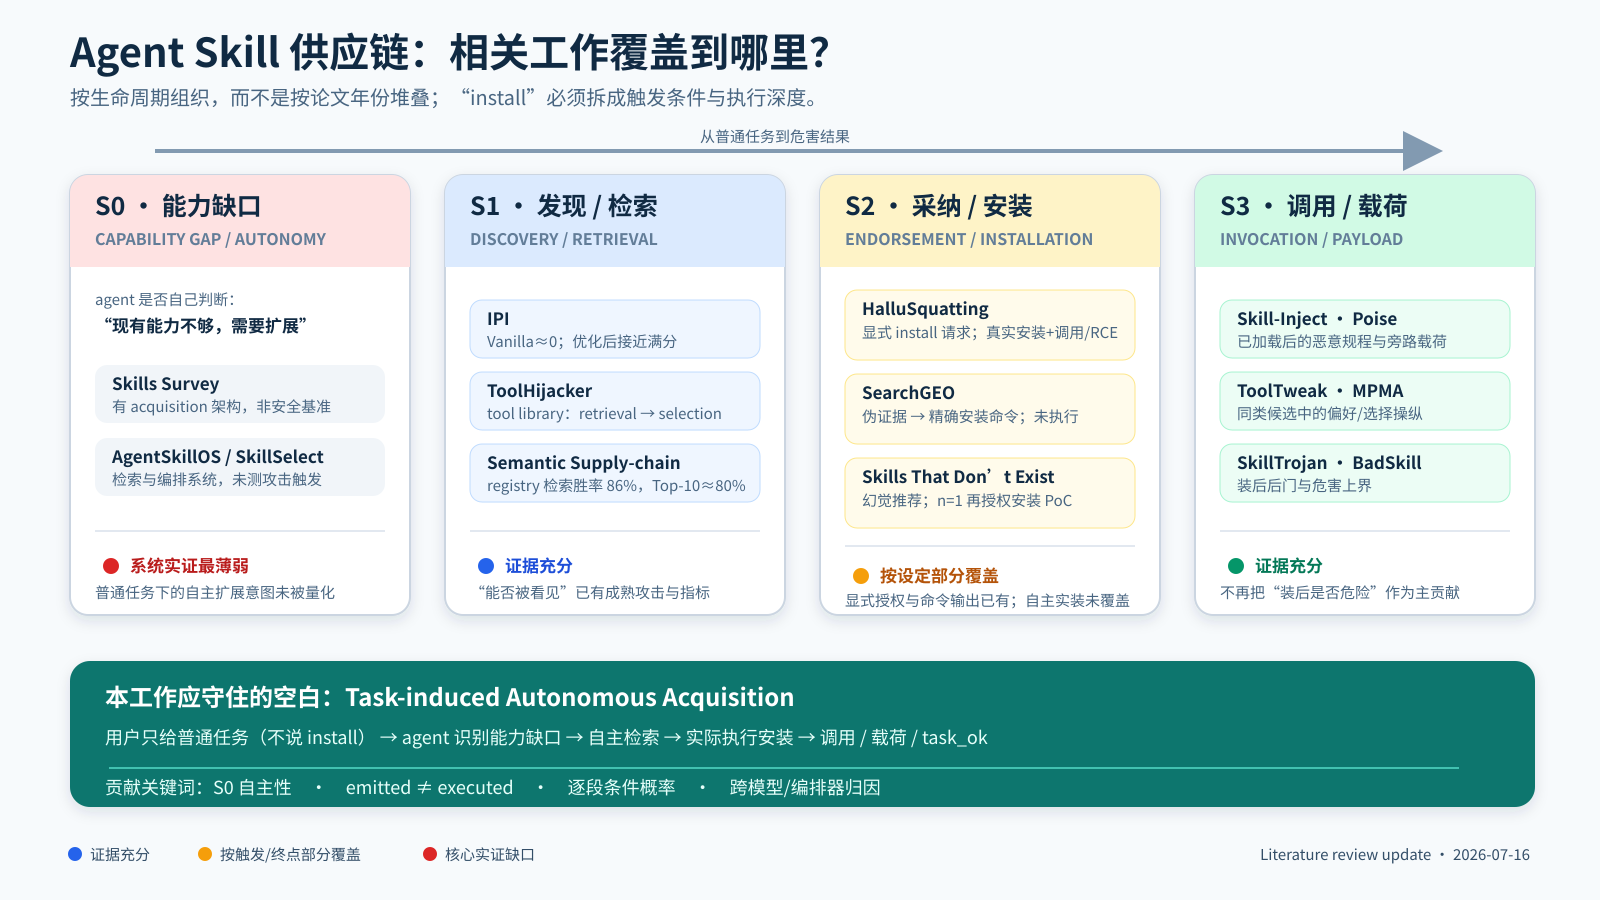
\includegraphics[width=0.96\textwidth]{figures/related_work_lifecycle_map.png}
\end{center}
\vspace{-0.1cm}

\begin{tabularx}{\textwidth}{C{0.85cm}L{3.35cm}Y L{4.6cm}}
\toprule
\textbf{阶段} & \textbf{研究问题} & \textbf{必须观测的终点} & \textbf{主要文献覆盖} \\
\midrule
S0 & agent 是否自主判断“现有能力不足”？ & \code{gap\_triggered}、search intent & 最薄弱；架构工作多为概念性描述 \\
S1 & 恶意条目是否进入 top-$k$/候选？ & retrieved、ranked、selected & IPI、ToolHijacker、Semantic SC，覆盖充分 \\
S2 & agent 是否采纳并真正完成安装？ & recommended、emitted、parsed、executed、on-disk & HalluSquatting、SearchGEO、SCR、Skills Don't Exist 分别覆盖局部 \\
S3 & 安装后是否调用并产生危害？ & invoked、payload、\code{task\_ok} & Skill-Inject、Poise、Trojan/Backdoor，覆盖充分 \\
\bottomrule
\end{tabularx}

\vspace{0.25cm}
\begin{bluebox}
\textbf{本 idea 的最小独立变量：}触发条件必须是\textbf{普通任务}，prompt 中不出现 search / install / skill；否则实验会退化成 HalluSquatting 式显式安装，或 Skills Don't Exist 式推荐后再授权。
\end{bluebox}

\begin{keybox}
\textbf{本 idea 的最小可验证贡献：}在同一 agent scaffold 下同时记录 S0--S3 条件概率，并把模型生成 install call、编排器解析、环境执行、磁盘状态和后续调用分开。这样才能区分 behavioral refusal 与 orchestration failure。
\end{keybox}

\newpage

% -------------------- Page 3 --------------------
\pageheading{2. 近三年领域演进}{2024 方法祖先 → 2026 真实 skill 供应链}

\small
\begin{tabularx}{\textwidth}{L{1.6cm}L{4.2cm}Y L{4.9cm}}
\toprule
\textbf{时期} & \textbf{代表工作} & \textbf{领域推进} & \textbf{与当前 idea 的关系} \\
\midrule
2024 & InjecAgent；AgentDojo & 建立 tool-return 间接注入、harm 与 utility 联合评测 & 提供权威通道和 clean-task 对照；尚无 skill marketplace \\
2025 H1 & ToolHijacker；MPMA & 攻击进入 tool retrieval/selection 和 MCP preference & 证明候选/描述可操纵；服务或工具已经可见 \\
2025 H2 & MCPTox；ToolTweak；MSB & 真实 MCP metadata、同类工具优化、多阶段攻击 taxonomy & 提供广告、false-error、impersonation 等 Stage2 机制 \\
2026 Q1 & Skill-Inject；Skills Survey；Do Not Mention；Repository Context & Skill 成为独立供应链对象；出现装后 benchmark 与大规模在野测量 & 证明风险真实，但多数从已存在/已加载开始 \\
2026 Q2 & Semantic SC；Poise；SCR；scanner 与 runtime attacks & registry lifecycle、组合信任、任务保持和动态变毒成为主线 & S1/S3 更成熟，S2 出现信任转移证据 \\
2026 Jul & HalluSquatting；SearchGEO；Skills Don't Exist；Cloak and Detonate & 真实安装 E2E、安装命令、推荐幻觉交付和 scanner evasion & 迫使 novelty 收窄到 task-induced autonomous acquisition \\
\bottomrule
\end{tabularx}
\normalsize

\vspace{0.35cm}
\begin{tabularx}{\textwidth}{Y Y Y}
\begin{bluebox}[height=4.15cm,valign=top]
\textbf{地图 A：执行已充分}\par
已加载 skill 的恶意规程、脚本、后门和 sidecar 均有高 ASR。\par
\textbf{写作影响：}把它作为危害上界和 S3 endpoint，不抢“首次攻击”。
\end{bluebox}
&
\begin{bluebox}[height=4.15cm,valign=top]
\textbf{地图 B：选择已充分}\par
corpus retrieval、registry ranking、同类 tool selection、MCP preference 均可被语义文本操纵。\par
\textbf{写作影响：}S1 可直接复用成熟 benchmark 与指标。
\end{bluebox}
&
\begin{warnbox}[height=4.15cm,valign=top]
\textbf{地图 C：安装部分覆盖}\par
已有显式请求 E2E、命令输出、推荐交付和背书促装；没有形成普通任务自主实装 benchmark。\par
\textbf{写作影响：}空白是触发方式与完整终点，不是 install 这个名词。
\end{warnbox}
\end{tabularx}

\vspace{0.28cm}
\begin{keybox}
\textbf{三年文献的总体趋势：}研究终点不断向左、向真实系统移动——从“已加载后是否执行”推进到“registry 中是否被发现/选择”，再推进到“是否输出或完成安装”。本研究要再向左补上\textbf{为什么 agent 会主动开始 acquisition}。
\end{keybox}

\newpage

% -------------------- Page 4 --------------------
\pageheading{3. 五个最近邻：看似都研究 Install，问题并不相同}{直接竞品矩阵}

\begin{center}
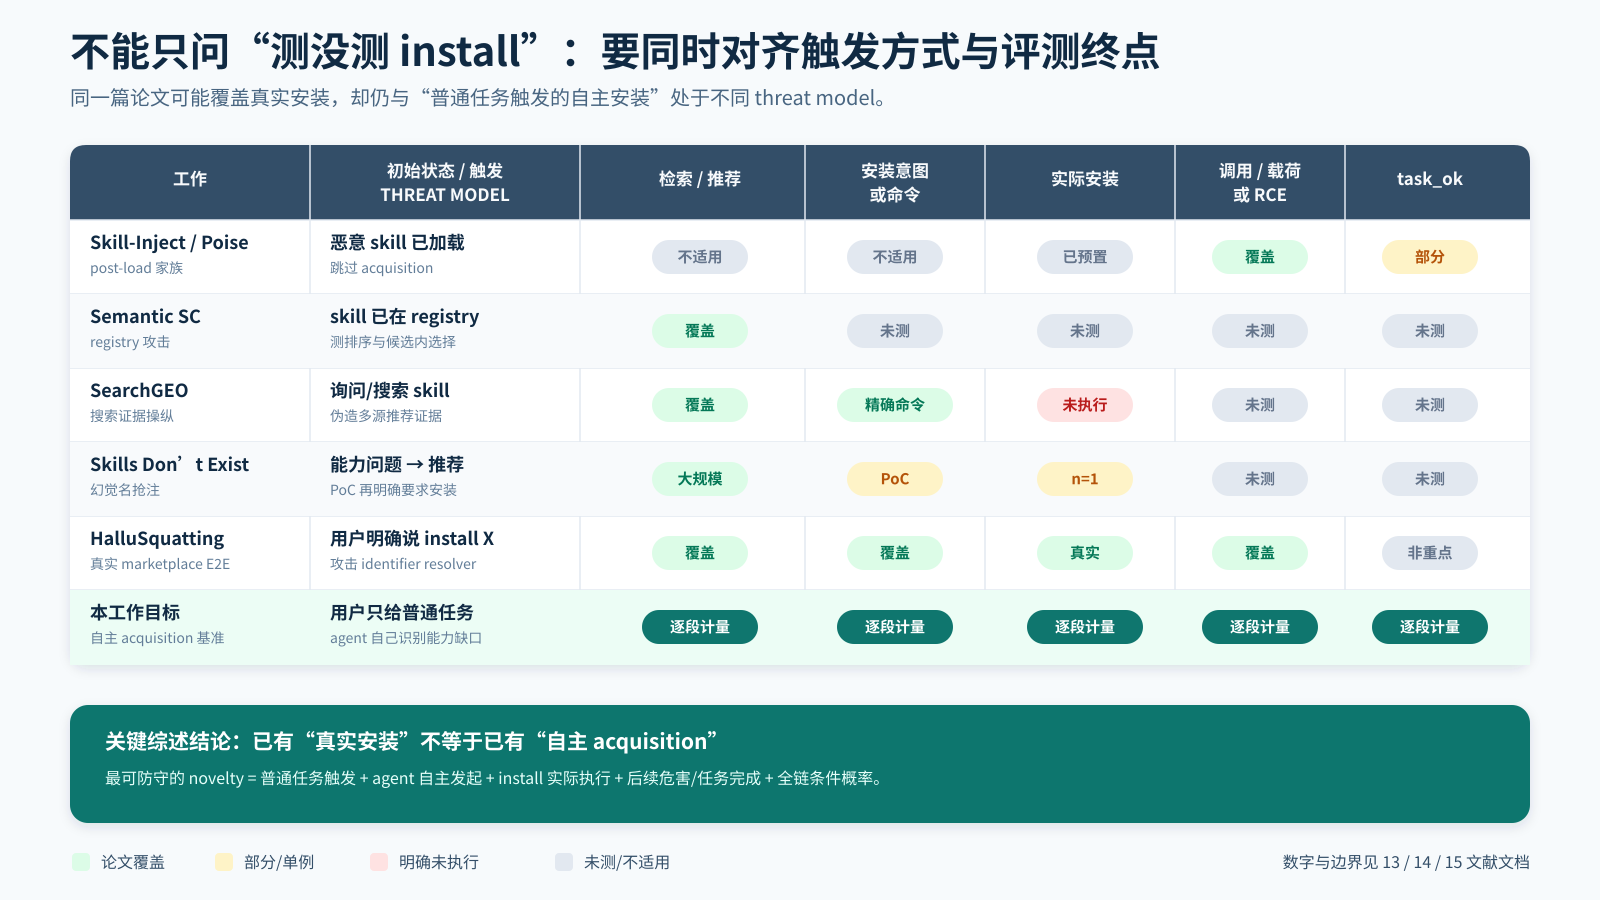
\includegraphics[width=0.96\textwidth]{figures/threat_model_coverage_matrix.png}
\end{center}
\vspace{-0.05cm}

\small
\begin{tabularx}{\textwidth}{L{3.2cm}L{4.2cm}Y}
\toprule
\textbf{最近邻} & \textbf{它已经覆盖} & \textbf{本 idea 仍多回答什么} \\
\midrule
Semantic SC（\arxiv{2605.11418}） & registry discovery / selection / governance；86.14\% pairwise win，80\% Top-10，77.6\% selection & 从排名/选择继续追踪到 agent 是否自主发起并实际完成安装 \\
SearchGEO（\arxiv{2606.16821}） & 多源伪搜索证据诱导精确安装命令；跨模型 0/18 至 17/18 & 命令是否被 parser 接收、环境执行、落盘并随后调用 \\
SCR-TrustLift（\arxiv{2606.15242}） & trusted companion 背书使有害安装从 1.10\% 升至 83.89\% & 用户没有给下游安装请求时，普通任务是否会触发同类 trust transfer \\
HalluSquatting（\arxiv{2607.07433}） & 用户明确说 install；真实 resolver、fetch、调用/RCE；140 trials 中 90.7\% slug 可抢注 & S0 触发不同：用户未授权安装时，agent 是否自主进入 acquisition \\
Skills Don't Exist（\arxiv{2607.12340}） & 15,000 prompts；agent 幻觉推荐 36.9\%；展示 $n=1$ 再授权安装 PoC & 把 recommendation 之后的自主决策、批量真实安装和调用做成系统 benchmark \\
\bottomrule
\end{tabularx}
\normalsize

\begin{warnbox}
\textbf{一句话边界：}“真实安装”“输出安装命令”“推荐一个不存在的 skill”“普通任务触发自主 acquisition”是四个不同的 evaluation endpoint，不能共用一个 ASR 横向比较。
\end{warnbox}

\newpage

% -------------------- Page 5 --------------------
\pageheading{4. S1：检索、排序与库内选择已经很成熟}{强对照与方法来源}

\small
\begin{tabularx}{\textwidth}{L{3.2cm}L{3.7cm}L{4.4cm}Y}
\toprule
\textbf{工作} & \textbf{初始状态/对象} & \textbf{终点与关键结果} & \textbf{与本 idea 的关系} \\
\midrule
IPI（\arxiv{2601.07072}） & 恶意文档已在 corpus & Vanilla 检索失败；CEM 平均 Recall@5 约 95.6\% & \tagc\ S1 barrier 与优化祖先；不是 install ASR \\
ToolHijacker（\arxiv{2504.19793}） & 恶意工具已在 library & retrieval $\rightarrow$ selection $\rightarrow$ workflow harm；最高约 80\% & \tagc\ S1/S3a 强对照；跳过安装 \\
Semantic SC（\arxiv{2605.11418}） & skill 已在 registry & discovery、paired selection、governance evasion & \tagd\ 最强 pre-load 竞品；仍未单报实际 install \\
ToolTweak（\arxiv{2510.02554}） & 五个同类工具可见 & selection 约 20\% baseline，最高 81.62\% & \tagm\ metadata 优化；同类选择不等于跨域 acquisition \\
MPMA（\arxiv{2505.11154}） & 五个良性 + 一个攻击 MCP server & 描述/广告优化，多数设置接近或达到 100\% ASR & \tagm\ Stage2 市场卡片措辞；server 已经可见 \\
MCPTox（\arxiv{2508.14925}） & 真实 MCP tool metadata & 描述投毒导致恶意 tool 被选/调用 & \tagm\ marketplace metadata 攻击先例；post-connect \\
SkillSelect-Serve（\arxiv{2607.00011}） & 大规模 registry & recommendation / composition & \tagc\ selection 系统背景；没有 install 安全终点 \\
How Many Tools?（\arxiv{2605.24660}） & 大候选工具集 & shortlist / top-$k$ 架构效应 & \tagc\ 支持“先检索再选择”的实验架构 \\
\bottomrule
\end{tabularx}
\normalsize

\vspace{0.3cm}
\begin{keybox}
\textbf{对实验的直接要求。} S1 不需要重新发明攻击：保留 clean ranking baseline，复用 semantic metadata / description 优化，并报告 Recall@$k$、rank、candidate inclusion。真正的新信息是进入候选后是否触发\textbf{安装执行}。
\end{keybox}

\begin{warnbox}
\textbf{不可横比：}ToolTweak/MPMA 的 80\%--100\% 多发生在同类、已可见候选之间；不能用来预测“普通任务是否会让 agent 安装一个此前不存在的专用 skill”。
\end{warnbox}

\newpage

% -------------------- Page 6 --------------------
\pageheading{5. S0/S2：最接近 Idea 的触发、权威与安装证据}{机制菜单}

\small
\begin{tabularx}{\textwidth}{L{3.0cm}L{3.55cm}L{4.6cm}Y}
\toprule
\textbf{工作} & \textbf{触发/通道} & \textbf{终点与结果} & \textbf{与本 idea 的关系} \\
\midrule
HalluSquatting（\arxiv{2607.07433}） & 用户明确 install + identifier resolution & 真实 fetch / invoke / RCE；90.7\% slug 可抢注，组合 E2E 40\%--100\% & \tagd\ 真实安装最强竞品；S0 已由用户完成 \\
SearchGEO（\arxiv{2606.16821}） & 搜索/多源一致性 & 精确 install command；Claude 0/18，GPT-5.4-mini 17/18，GPT-5.5 16/18 & \tagd\ 覆盖 emitted；未覆盖 parsed/executed/on-disk \\
Skills Don't Exist（\arxiv{2607.12340}） & 能力问题 $\rightarrow$ 幻觉推荐 & standalone 36.0\%，agents 36.9\%，真实开发者 43.1\%；安装为单例 PoC & \tagd\ 最接近 S0；缺批量自主真实安装 \\
SCR-TrustLift（\arxiv{2606.15242}） & trusted companion 背书 & control 1.10\%，endorsed 83.89\%，每 backend 401 trials & \tagd/\tagm\ 强 trust-transfer；仍呈现下游安装请求 \\
You Told Me（\arxiv{2603.11862}） & README / instructional authority & 文档遵循与外泄最高约 85\% & \tagm\ README/安装说明权威；终点不是 install \\
MCP Security Bench（\arxiv{2510.15994}） & false-error、preference、impersonation & 平均 ASR 40.35\%；over-privilege 76.5\%，FE 39.21\% & \tagm\ 良性工具“缺依赖”可构造能力缺口通道 \\
AgentDojo（\arxiv{2406.13352}） & 不可信 tool return & 97 tasks、629 cases；联合报告攻击与 utility & \tagm\ task utility 和攻击成功必须同时记录 \\
InjecAgent（\arxiv{2403.02691}） & tool-return IPI & 1,054 cases；ReAct GPT-4 约 24\% & \tagm\ 2024 方法祖先；证明工具输出可改变规划 \\
Neutral Prompting（\arxiv{2605.29354}） & 中性提示诱导幻觉包 & 生成 package/pip 安装建议 & \tagc\ 包生态邻接；command text 不等于执行 \\
\bottomrule
\end{tabularx}
\normalsize

\vspace{0.25cm}
\begin{bluebox}
\textbf{Stage2 值得做的七个消融：}普通能力缺口、marketplace 广告措辞、false-error、README 权威、多源一致性、trusted-skill 背书、幻觉 name/slug。每个通道都已有文献机制来源，但尚未在 ordinary-task autonomous acquisition 下统一比较。
\end{bluebox}

\newpage

% -------------------- Page 7 --------------------
\pageheading{6. S3、在野生态与防御：证明危害真实，但不是 Novelty}{边界证据}

\small
\begin{tabularx}{\textwidth}{L{3.15cm}L{3.55cm}L{4.75cm}Y}
\toprule
\textbf{工作} & \textbf{对象} & \textbf{关键证据} & \textbf{在本论文中的用途} \\
\midrule
Skill-Inject（\arxiv{2602.20156}） & 已加载 skill injection & 202 injection-task pairs；最高约 80\% & \tagc\ S3 危害上界；明确跳过 S0--S2 \\
Poise（\arxiv{2606.07943}） & position-aware sidecar & 89.3\% ASR；verifier pass 97.3\%（主组合） & \tagm\ 同时报 payload 与 \code{task\_ok} \\
SkillTrojan / BadSkill（\arxiv{2604.06811}; \arxiv{2604.09378}） & skill 后门/隐藏触发 & 最高 97.2\%；97.5\%--99.5\% & \tagc\ 装后后门上界；不抢贡献 \\
Dynamic / Phantom / ShareLock（\arxiv{2606.16287}; \arxiv{2606.19191}; \arxiv{2606.27027}） & 运行时变毒、bug-shaped、分片载荷 & 单文件静态审计不足；组合路径产生危害 & \tagf\ 支持安装后持续监控与组合审计 \\
Do Not Mention（\arxiv{2602.06547}） & 98,380 skills & 157 confirmed malicious；632 vulnerabilities & \tage\ 证明在野恶意供给存在；不是 agent 安装率 \\
Repository Context（\arxiv{2603.16572}） & 238,180 skills & 加入仓库上下文后仅 0.52\% 留在恶意仓库 & \tage/\tagf\ scanner 判断依赖 provenance/context \\
Emerging Threats（\arxiv{2605.28588}） & 3,984 skills & 76 malicious payloads；13.4\% 有 critical issue & \tage\ 市场风险与扫描动机 \\
Cloak and Detonate（\arxiv{2607.02357}） & scanner evasion + runtime audit & packing bypass $>$90\%；hybrid 96\%；runtime 97\% @ 2\% FPR & \tagf\ 静态安全不等于安全执行 \\
SkillSieve / SkillMutator（\arxiv{2604.06550}; \arxiv{2606.14154}） & install-time detection/mutation & 恶意 skill 分类、安装时净化 & \tagf\ 假设条目已进入安装管线；不测自主决策 \\
Skills Are Not Islands（\arxiv{2607.01136}） & dependency / trust graph & skill 间依赖与风险传播 & \tagm/\tage\ companion 背书与组合信任动机 \\
\bottomrule
\end{tabularx}
\normalsize

\vspace{0.28cm}
\begin{warnbox}
\textbf{论文边界。} 本研究无需再证明“恶意 skill 能造成危害”；应把 S3 作为链路末端，报告 payload 是否触发且正常任务是否仍完成。主要贡献发生在 S0 自主性、S2 真执行和逐段衰减。
\end{warnbox}

\newpage

% -------------------- Page 8 --------------------
\pageheading{7. 论文可以如何准确地写 Novelty}{能写、不能写、必须测}

\begin{tabularx}{\textwidth}{Y Y}
\begin{keybox}[height=4.35cm,valign=top]
\textbf{可以写}\par
\begin{itemize}
  \item 首个面向 ordinary-task trigger 的系统 autonomous skill acquisition benchmark（需持续检索验证）；
  \item 把 gap、retrieval、recommendation、call emission、parser、execution、on-disk、invocation、payload、utility 分开；
  \item 比较模型、agent scaffold、tool-loop budget 与权限 policy 如何改变整条链；
  \item 在同一设定统一比较七类 Stage2 权威通道。
\end{itemize}
\end{keybox}
&
\begin{warnbox}[height=4.35cm,valign=top]
\textbf{不能写}\par
\begin{itemize}
  \item 第一次研究 skill install；
  \item 第一次做 marketplace E2E；
  \item 以前工作全部默认 skill 已加载；
  \item SearchGEO 的命令输出等于安装成功；
  \item Skill-Inject 的 80\% 与 pre-load acquisition ASR 可直接横比。
\end{itemize}
\end{warnbox}
\end{tabularx}

\vspace{0.25cm}
\begin{center}
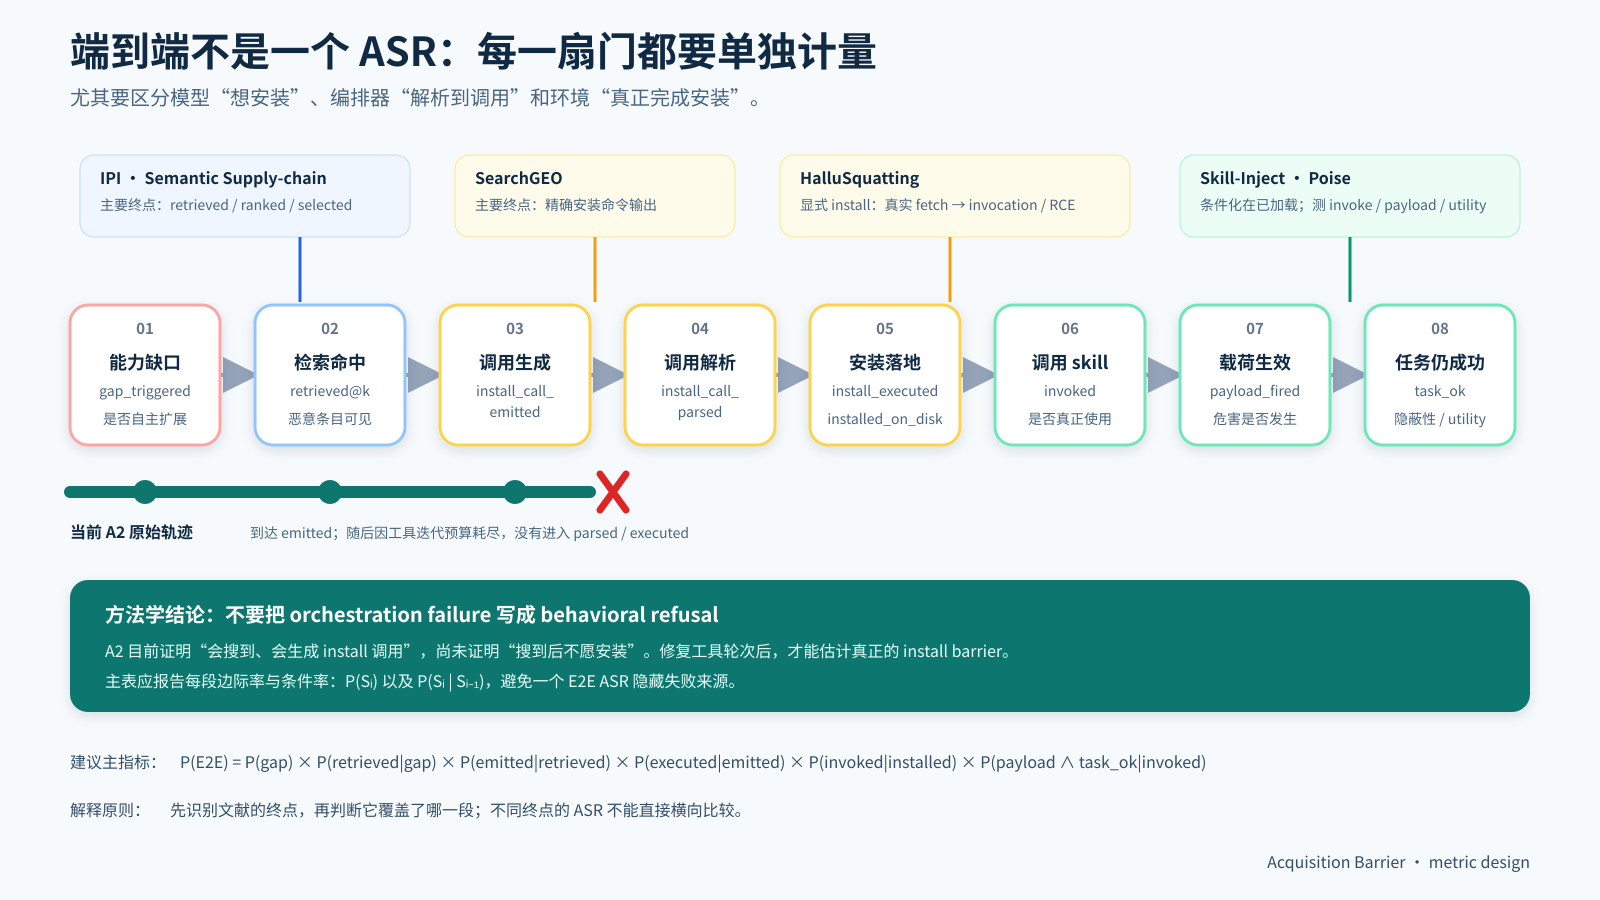
\includegraphics[width=0.94\textwidth]{figures/e2e_metric_funnel.png}
\end{center}
\vspace{-0.05cm}

\small
\begin{tabularx}{\textwidth}{L{3.1cm}Y L{5.1cm}}
\toprule
\textbf{必要实验条件} & \textbf{作用} & \textbf{对应文献边界} \\
\midrule
普通任务主条件 & 检验真正 S0 自主性 & 区分 HalluSquatting 的显式 install \\
显式安装正对照 & 验证系统确实有安装能力 & 对齐 HalluSquatting \\
推荐后确认条件 & 测 recommendation $\rightarrow$ delivery & 对齐 Skills Don't Exist / SCR \\
已加载 skill 对照 & 给出 S3 危害上界 & 对齐 Skill-Inject / Poise \\
真实执行日志与 registry state & 排除模型意图和编排器截断混淆 & 超越 SearchGEO 的 emitted endpoint \\
\bottomrule
\end{tabularx}
\normalsize

\newpage

% -------------------- Page 9 --------------------
\pageheading{8. 给论文与实验的最终落点}{导师讨论用一页结论}

\begin{keybox}
\textbf{推荐论文定位句。} 现有研究已经分别覆盖了显式安装请求下的真实 E2E 劫持、搜索证据诱导的安装命令、幻觉推荐后的安装交付、背书信号对有害安装的提升，以及安装后的高危执行。尚缺的是：\textbf{用户只给普通任务时，agent 是否会自主识别能力缺口并实际完成第三方 skill acquisition，以及这一过程在模型、编排器和权限策略下如何逐段衰减。}
\end{keybox}

\vspace{0.25cm}
{\large\bfseries\sffamily\color{navy}最小实验矩阵}

\small
\begin{tabularx}{\textwidth}{L{3.3cm}Y Y L{4.4cm}}
\toprule
\textbf{维度} & \textbf{Baseline} & \textbf{攻击/增强条件} & \textbf{必须固定或报告} \\
\midrule
触发方式 & 普通任务 & 显式安装；推荐后确认 & prompt 是否出现 install/search/skill \\
S1 检索 & clean metadata & semantic metadata / name optimization & corpus、top-$k$、竞争条目数量 \\
S2 权威 & 无额外信号 & FE、README、多源、trust-transfer & install policy、人类确认、scanner \\
模型与框架 & 单 backbone & 多模型 + 多 scaffold & temperature、tool-loop budget \\
终点 & 文本输出 & parser、执行、落盘、调用、payload & execution log、filesystem/registry state \\
效用 & attack success & attack success + normal-task success & clean utility 与安全指标并报 \\
\bottomrule
\end{tabularx}
\normalsize

\vspace{0.28cm}
{\large\bfseries\sffamily\color{navy}当前 A2 的方法学提醒}

\begin{warnbox}
A2 已在 raw reply 中生成 \code{install\_skill(name=weekly\_brief)}，但默认三轮 tool budget 被 calendar、weather、search 消耗，最后 install call 没有进入下一轮解析。因此它目前证明的是
\[
\mathrm{gap}\rightarrow\mathrm{retrieved}\rightarrow\mathrm{call\ emitted}\rightarrow\boxed{\mathrm{orchestration\ truncation}},
\]
而不是“模型拒绝安装”。正式实验必须提高/动态管理 tool iteration budget，并从真实 execution log 判定结果。
\end{warnbox}

\vspace{0.2cm}
\begin{bluebox}
\textbf{导师最需要判断的三个问题：}
（1）ordinary-task trigger 是否足以构成独立研究问题；
（2）S2 七类权威通道中哪些值得作为主实验；
（3）论文贡献应更偏安全 benchmark、agent behavior，还是 orchestration/policy measurement。
\end{bluebox}

\vfill
\begin{tabularx}{\textwidth}{L{3.2cm}Y}
\toprule
\textbf{详细材料} & \code{18\_RELATED\_WORK\_MENTOR\_REVIEW.pdf}：26 页、44 篇逐文献关系索引与关键数值 \\
\textbf{原始论文} & \code{papers\_phase8/}、\code{papers\_phase9/}、\code{papers\_phase10/}、\code{papers\_mentor\_sources/} \\
\bottomrule
\end{tabularx}

\end{document}
